\documentclass[10pt, a4paper]{article}
\usepackage{lrec}
\usepackage{multibib}
\newcites{languageresource}{Language Resources}
\usepackage{graphicx}
\usepackage{tabularx}
\usepackage{soul}
\usepackage{color}
% for eps graphics

\usepackage[normalem]{ulem}

\usepackage{epstopdf}
\usepackage[utf8]{inputenc}

\usepackage{hyperref}
\usepackage{xstring}

\newcommand{\secref}[1]{\StrSubstitute{\getrefnumber{#1}}{.}{ }}

\title{Transformation-based Annotation of Norm Deviations \\ in an Infrastructure for Research on Swedish as a Second Language}

\name{Author1, Author2, Author3}

\address{Affiliation1, Affiliation2, Affiliation3 \\
         Address1, Address2, Address3 \\
         author1@xxx.yy, author2@zzz.edu, author3@hhh.com\\
         \{author1, author5, author9\}@abc.org\\}

\abstract{
This paper describes ongoing work on the development of an infrastructure for research on Swedish as a second language, with particular focus on our system for annotation of deviations (errors) relative to the norm of the language being learned. Unlike traditional approaches which treat this as a single task applied to a static learner text, our approach is divided into two successive steps to reflect the conceptual structure of the problem: a) normalisation  of the learner text by transforming (editing) it to reflect the target hypotheses, and b) the actual norm-deviation annotation, supported by visualisation of the differences between source and normalisation. An additional advantage of our approach is that a parallel text is generated in the transformation step, with word alignments inferred from the editing operations. This is a useful resource in its own right, by allowing for search of both the source and normalised texts, and for training of systems for automated annotation of norm deviations. We describe the overall design of the transformation-based annotation system, as well as the workflow and initial user experiences [179 words out of 200 allowed].}

\begin{document}

\maketitleabstract

\section{Background and Introduction}

SweLL project focuses on setting up an electronic research infrastructure for Swedish as a Second Language. In general terms, an electronic research infrastructure ideally consists of:
\begin{enumerate}
\item  (free accessible) data in electronic format
\item  technical platform for exploring the data, including tools and algorithms for data analysis,  and visualization
\item a set of tools and technical solutions for new data collection and preparation, including data processing and annotation
\item  relevant expertise within the area
\end{enumerate}


The need for data is omnipresent within Language Technology projects, and not the least when it comes to data produced by second language (L2) learners. Not only the L2 data is sensitive in nature and requires (agreements for use of) associated socio-demographic information, but it also demonstrates a good deal of deviations from the language norms to be analyzed with existing NLP tools. Preparation of L2 data for NLP experiments is therefore very demanding, where annotation of norm deviations (error annontation) is probably the most time-consuming step.

 \ldots

One focus of the current work is annotation of norm deviations in L2 texts. \ldots

\section{Transformation-based Annotation}

Annotation of norm deviations in second-language learner texts (traditionally called error annotation) is typically done with a purpose-built editing tool, using a hierarchical set of error categories (Granger 2009). For example, in ASK (Tenfjord et al. 2006), the editor used is Oxygen (https://www.oxygenxml.com), an XML editor which has been customised with pop-up menus that reflect the chosen set of error categories. Specifically, annotation of an error involves inserting an XML {\em sic} tag with a {\em type} attribute encoding the error category, a {\em desc} attribute endoding the error subcategory, and a {\em corr} attribute encoding the correct (normalised) form of the token or tokens. The XML annotation can be translated to a presentation format in HTML which can be viewed in a web browser, thereby facilitating proofreading.

The basic problem with this kind of approach is that it conflates the conceptually separate stages of (traditionally speaking) error coding, namely, error detection, correction and annotation (Corder 1974, Ellis 1994, Granger 2009, page 266). This is because correction (normalisation, based on a target hypothesis) is carried out as a subtask of error annotation instead of as an independent task, prior to and separate from error annotation. Also, since normalisations are only a by-product of error annotations, the corrected text as a whole is not available for inspection after each successive correction step, and it may therefore be more difficult to produce a reliable and consistent normalisation.

In Falko (L{\"u}deling et al.\ 2005) and MERLIN (MERLIN project 2014), target hypothesis corrections have a more independent status in the sense that they are entered in a separate step prior to error annotation, but the normalised text still does not seem to be available in its entirety. To circumvent these problems, our approach is based on dividing error coding into two steps: normalising the text by transforming (editing) it into a corrected form according to some guideline, and annotating the norm deviations corresponding to the changes.

\subsection{Target Hypotheses and Normalisation}

Normalisation involves, for each deviation from the norm, to decide on a target hypothesis and to edit the text to mirror this hypothesis. We take an editing operation to be insertion, deletion, replacement \textcolor{red}{EV:("substitution" instead of "replacement"?; merge? split? - separate actions or as variants of replacement, insertion and deletion?)} and move \textcolor{red}{EV:(Is it a term?)}
of one or several tokens \textcolor{red}{(EV: what about characters?)}. By keeping track of the sequence of such editing operations, an additional advantage could be gained, namely, that a basic, preliminary error annotation could be automatically inferred. We plan to explore this possibility later in the project.

To facilitate normalisation and to support reliability and consistency,
we use three panes (see Figure~\ref{fig:screenshot}): one containing the
frozen source text, one in which the editing takes place, and one in which
changes are highlighted. It might be argued that insertions, deletions and
replacements could be calculated automatically from the differences between
the source and normalised texts without logging the editing operations, but
moves of tokens (which we need in order to keep track of word-order changes)
is more difficult to calculate, which is why we log the editing operations.

\begin{figure*}
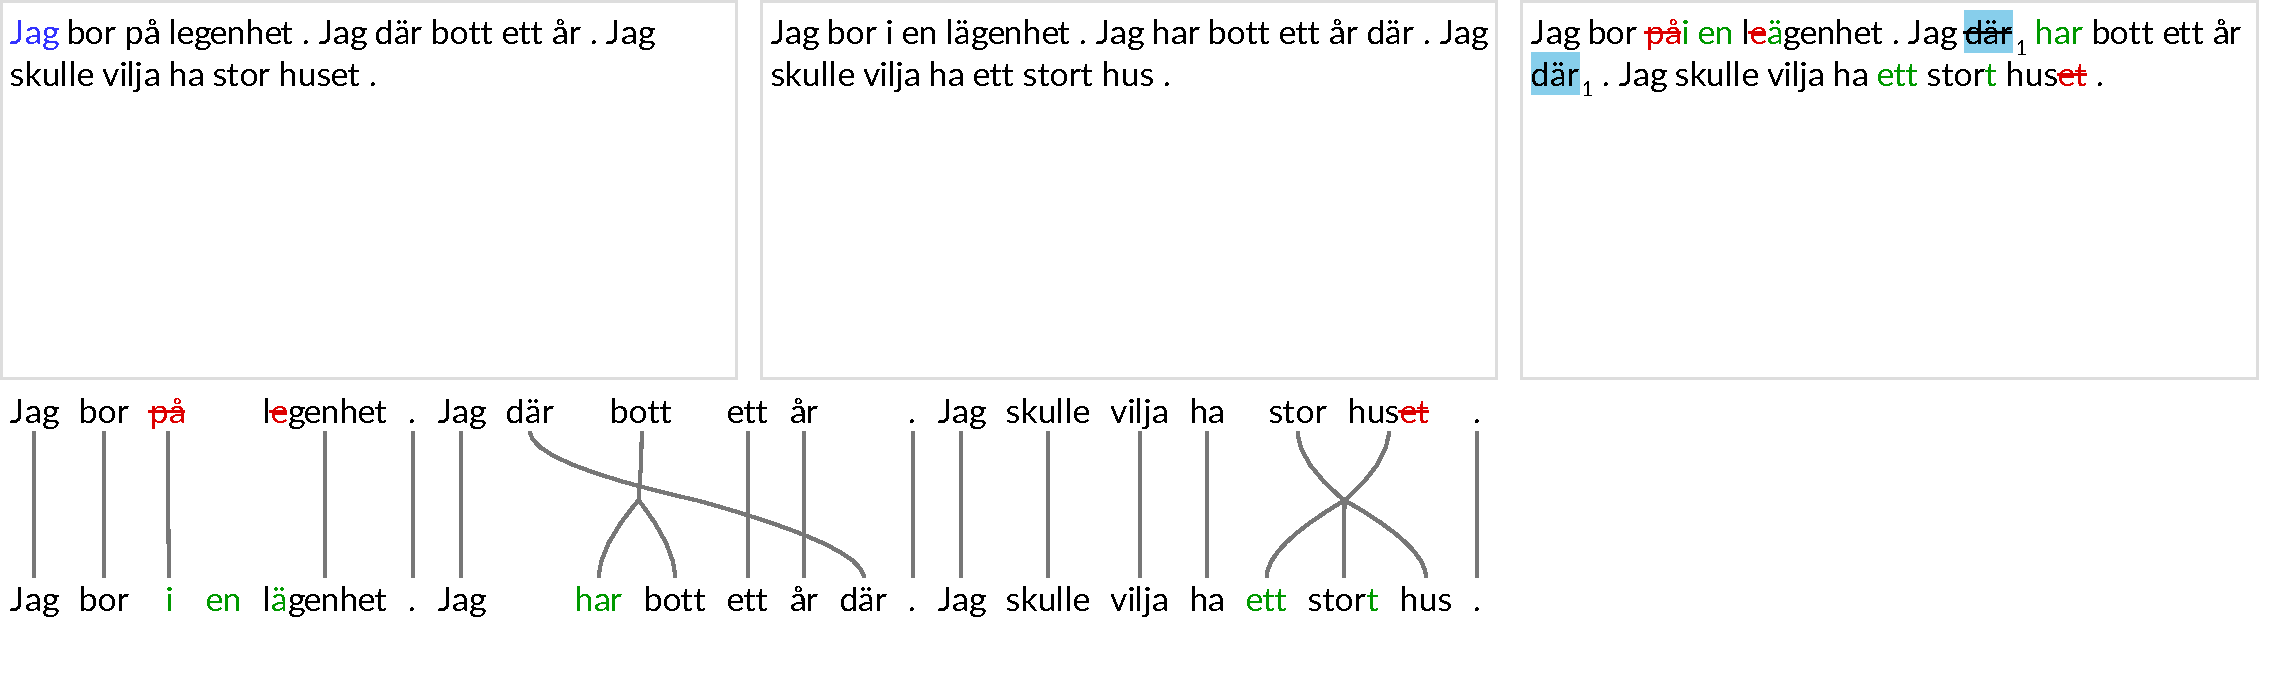
\includegraphics[width=\textwidth, trim={0 1cm 0 0}, clip]{screenshot.pdf}
\emph{\small I live in an apartment. I have lived there for one year. I would like to have a big house.}
\caption{Screenshot of an editing session in progress. The three panes in the upper row are from left to right:
1) the source text which cannot be edited,
2) the target hypothesis which is where the annotator do all their edits,
3) a calculated view of the differences between the two texts obtained from the history of edits.
Below the panes we display the the differences pictorially:
the source text on top and the target hypothesis below, with edges
showing how words have been moved.
% Deletions are shown in \textcolor{red}{red} with \sout{overstrike},
% insertions in \textcolor{green}{green} with \underline{underline}.
% (If the text is too long only the current sentence is shown.)
\label{fig:screenshot}
}
\end{figure*}

% Should this be here or in related work? I added a blurb about Hana et al's work /Dan
Some systems allow for multiple (vertical) levels of target hypotheses. In the Czech learner corpus of \newcite{Hana2014} a
first level normalises grammatical forms without context information. All other deviations (e.g. word order) belong to a second level and take the whole sentence into consideration.
In MERLIN (MERLIN project 2014) two levels are used: a) minimal corrections pertaining only to orthographic and grammatical errors and b) corrections to handle sociolinguistic, lexical and pragmatic deviations to arrive at what is referred to as an acceptable text. This could be handled in our approach by maintaining several levels of aligned normalisations. The first level (with basic corrections) would then be aligned to the source text, and the second level (with additional corrections) would be aligned to the first level. Adding several levels is something that we have not undertaken yet, however. We also do not handle multiple {\em competing} target hypotheses for the same source material in the manner of L{\"u}deling et al. (2005) \textcolor{red}{(EV: should also provide page)}.\footnote{An example of this from L{\"u}deling et al. (ibid.) is "diese Ph{\"a}nomen" which could be interpreted either as a gender error (with the target hypothesis "dieses Ph{\"a}nomen") or as a number error (with the target hypothesis "diese Ph{\"a}nomene").} In principle, this could be handled in our approach by maintaining different normalisations on the same level for a given part of the source text.

\section{Design of our normalisation tool}

We set off to build a normalisation tool to be both simple and expressive.
We wanted it to have the feel of a conventional text editor and yet retain
information about how a word was normalised or where it was moved to. To be
able to answer questions about movement we make the assumption that the text
can be tokenized. For now we assume that tokens are separated by whitespace
and cannot contain whitespace themselves. Thus inserting whitespace between
characters makes a new token and deleting the last whitespace between two
tokens merges them into one.

% Where should this paragraph be?
We assume that the user can during normalisation be required to pay attention
to how their edits affect the links between the source text and the target
hypothesis. We facilitate this by providing views of their difference and
the links between them.

For expressing overcompounding and oversplitting we need links between tokens
that are many-to-one and one-to-many. We express insertion or deletion with
zero-to-one and one-to-zero links. We initially experimented with not allowing
many-to-many links but this asymmetry yielded no substantial benefits
and we now allow many-to-many links.
% of which we outline some benefits of below
For simplicity we require each component
of links must be complete: missing edges are automatically added by
transitivity.

We now outline how to instrument a traditional text editor to support links.
When starting the editing session the source and target are identical so the
links are initialised with the identity mapping. The user starts editing
by inserting and deleting characters.
We generalizing this to each edit which replaces the current selection with a
string. Usually the selection is just the cursor and the ``replacement'' string
is one character: then the modification is an insertion.
If the selection has non-zero width the user did an actual replacement.
Deletions are modelled by replacing with the empty string.
%The inserted string can also have length greater than one if the user pastes text into the editor.

When the editor is linked to a source text we also need to update the links.
This is how to resolve the possible editing situations:
% Could make images for each and every one of these (but what example texts to use?)

\begin{itemize}

\item {\it Edit within an existing token:}
Update the target word, links stay the same.

\item {\it Edit ranging over several tokens:}
Merge the links from the involved tokens and update the text.

\item {\it Edit removing a token completely:}
Removes any links from the source to this target token.
If this removes the last link of a source token it means that
it is deleted in the hypothesis (presumably a redundant word.)

\item {\it Edit introducing new whitespace:}
The user wants to split a word, perhaps an overcompound.
Pass over all links form the token to each new token.
% Can introduce unlinked tokens (insertions) as a special case, could come back to this

\end{itemize}

The above outline handles most common edit operations, and includes derived
operations such as search and replace which can be seen as a sequence of edits.

We support rearranging the words by making cut and paste aware of the link
structure. To move a sequence of words the user selects a range
which includes these words and presses the shortcut for cutting: {\it Ctrl+X}.
This does not yet cut the words but instead highlights them. We expand partially
selected tokens to whole tokens to simplify this operation. The user then
navigates to the position they want the words to go and press the paste
shortcut: {\it Ctrl+V}.
This moves the tokens together with their links to the new position.
This rearranging operation can also be executed with the mouse using drag and drop.
% Image with example showing this step by step?

\subparagraph{Undo} We support unlimited chronological undo and redo.
For convenience we also support undo at a specific position. % in the hypothesis.
If this position is part of a compound of the entire compound is reverted.
Tokens are rearranged into their original positions, which
can be recovered using unmoved words as reference points.
Undoing is very useful to get links exactly right, which occasionally takes a
few tries.
% Auto-revert: we automatically auto-revert compounds if the user writes them
% back to the original

\subparagraph{Intra-token diffs} We show differences inside tokens by
calculating a diff automatically using standard techniques for finding
edit scripts.  Deletions are shown in red with overstrike and insertions
in green.  Note that this intra-token diff is recalculated after every edit
as interntally only replacements on the token level are stored.  However,
this clear highlighting of differences works as an aid for the user.

\paragraph{Implementation}
We have implemented a working prototype as a single-page web application.
It does not rely on any server backend: all processing is done in the
client's browser. We use an off-the-shelf editor for web applications,
CodeMirror\footnote{\url{https://codemirror.net}},
instrumented as described in this section.
Internally we keep an array of the tokens in the target text together with
which indexes of the source tokens it links to.  We only use immutable data
structures for ease of implementation,  which could be an efficiency problem:
it makes makes array operations linear in the length of the text. Should
this prove too slow for long texts it can be improved by restricting move
operations to only be within, say, paragraphs. Another alternative is to
switch to a more sophisticated data structure such as sequences built on
top of finger trees, which admit updates in logarithmic time.

\section{Annotation of Norm Deviations}

%
We want to support annotating the edits from the normalisation with a taxonomy
of norm deviations.  The intent is to put labels on components of links.
This can be done after normalising the text, but we can go back and forth
between the modes if the annotator want to improve the normalisation.

Note to reviewers: this is the scheduled to be completed in a few weeks
will be completed well before the camera-ready version.
%

Elena: Also something about about our intended error categories?

\section{Discussion}

Summarise overall workflow\ldots ?

We believe that the following properties of our approach will contribute to more reliable normalisation, less time-consuming annotation and production of more valuable corpus resources compared to traditional methods (can we substantiate any of this?):

First, the conceptually different tasks of deciding on a target hypotheses (with resulting normalisations) and annotating norm deviations are separated. Also, since the source text and normalised text are displayed in separate panes, with the normalised text being incrementally updated, the annotator is provided with excellent facilities for getting to know the specific inter-language of the learner, and to make consistent decisions on target hypotheses. In addition, the editing operations could be used for inferring a preliminary error annotation, though this is a path that we have not yet explored. Furthermore, a parallel text is automatically constructed based on the editing operations, which provides a resource valuable for independent purposes, such as training of a system for automated normalisation.

The user experience will be improved by allowing the annotator to connect
and disconnect links directly in the ladder diagram. This should also be
possible by using keyboard shortcuts in the editor.  Frequent operations
such as transposing words can also get dedicated keyboard bindings.

\section{Conclusion}

Your submission of a finalised contribution for inclusion in the LREC
proceedings automatically assigns the above-mentioned copyright to ELRA.

\section{Acknowledgements}

Place all acknowledgements (including those concerning research grants and
funding) in a separate section at the end of the article.

\section{Providing References}

\subsection{Bibliographical References}
Bibliographical references should be listed in alphabetical order at the
end of the article. The title of the section, ``Bibliographical References'',
should be a level 1 heading. The first line of each bibliographical reference
should be justified to the left of the column, and the rest of the entry should
be indented by 0.35 cm.

The examples provided in Section \secref{main:ref} (some of which are fictitious
references) illustrate the basic format required for articles in conference
proceedings, books, journal articles, PhD theses, and chapters of books.

\subsection{Language Resource References}

Language resource references should be listed in alphabetical order at the end
of the article, in the \textbf{Language Resource References} section, placed after
the \textbf{Bibliographical References} section. The title of the ``Language Resource
References'' section, should be a level 1 heading. The first line of each
language resource reference should be justified to the left of the column, and
the rest of the entry should be indented by 0.35 cm. The example in Section
\secref{lr:ref} illustrates the basic format required for language resources.

In order to be able to cite a language resource, it must be added to
the \texttt{.bib} file first, as a \texttt{@LanguageResource} item type, which
contains the following fields:

\begin{itemize}
    \item{\texttt{author}: the builder of the resource}
    \item{\texttt{title}: the name of the resource}
    \item{\texttt{publisher}: the publisher of the resource (project,
          organisation etc)}
    \item{\texttt{year}: year of the resource release}
    \item{\texttt{series}: more general resource set this language resource
          belongs to}
    \item{\texttt{edition}: version of the resource}
    \item{\texttt{islrn}: the International Standard Language Resource Number
          (ISLRN) of the resource\footnote{The ISLRN number is available from
          \texttt{http://islrn.org}}}
\end{itemize}

If you want the full resource author name to appear in the citation, the
language resource author name should be protected by enclosing it between
\texttt{\{...\}}, as shown in the model \texttt{.bib} file.

\vspace{.3\baselineskip}

\section*{Appendix: How to Produce the \texttt{.pdf} Version}

In order to generate a PDF file out of the LaTeX file herein, when citing
language resources, the following steps need to be performed:

\begin{itemize}
    \item{Compile the \texttt{.tex} file once}
    \item{Invoke \texttt{bibtex} on the eponymous \texttt{.aux} file}
    \item{Invoke \texttt{bibtex} on the \texttt{languageresources.aux} file}
    \item{Compile the \texttt{.tex} file twice}
\end{itemize}

% \nocite{*}
\section{Bibliographical References}
\label{main:ref}

\bibliographystyle{lrec}
\bibliography{xample}


\section{Language Resource References}
\label{lr:ref}
\bibliographystylelanguageresource{lrec}
\bibliographylanguageresource{xample}

\end{document}
